% !TeX spellcheck = de_CH_frami

\section{MOS-Transistor als Stromquelle (Kap. 8)}
Die Drain-Source-Strecke des MOS-Transistors stellt im Sättigungsbetrieb eine gesteuerte Stromquelle dar, deren Ausgangswiderstand (Innenwiderstand am Drain) relativ hoch ist.\\
\begin{minipage}[c]{0.45\textwidth}
	\subsection{Strom einer MOS Stromquelle}
	$I_D=\frac{\beta}{2}(V_{GS}-V_T)^2\textcolor{gray}{(1+\lambda V_{DS})} \approx \frac{\beta}{2}(V_{GS}-V_T)^2$\\
\end{minipage}
\begin{minipage}[c]{0.55\textwidth}
	\subsection{Sättigungsspannung}
	\textbf{Bei starker Inversion} $V_{DS} \geq V_{DS,sat}=V_{GS}-V_T=\sqrt{\frac{2I_D}{\beta}}$\\
	\textbf{Bei schwacher Inversion} $V_{DS} \geq V_{DS,sat}\approx 5\Phi_t \approx \SI{130}{\milli\volt}$
\end{minipage}\\
\begin{tabular}{|p{0.3025\textwidth}|p{0.3025\textwidth}|p{0.3025\textwidth}|}
	\hline
	\textbf{einfache Stromquelle mit und ohne Source-Widerstand}&\textbf{Stromquelle mit Kaskode}&\textbf{Stromquelle mit geregelter Kaskode}\\
	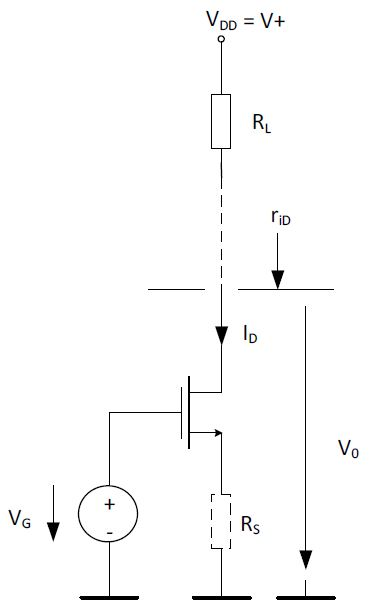
\includegraphics[height=4.5cm]{chapters/Stromquelle/images/einfacheStromquelle}&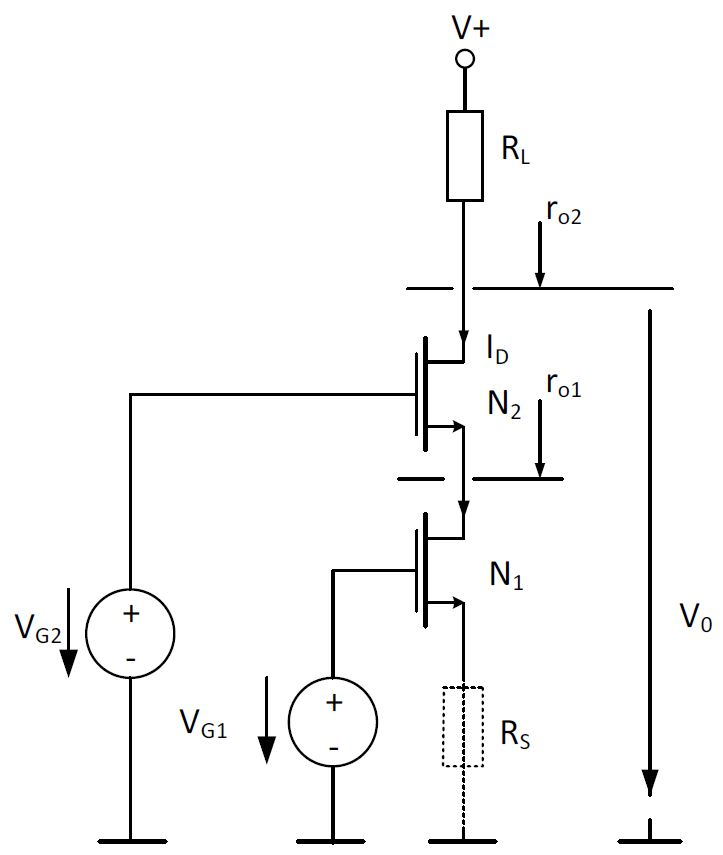
\includegraphics[height=4.5cm]{chapters/Stromquelle/images/Kaskode}&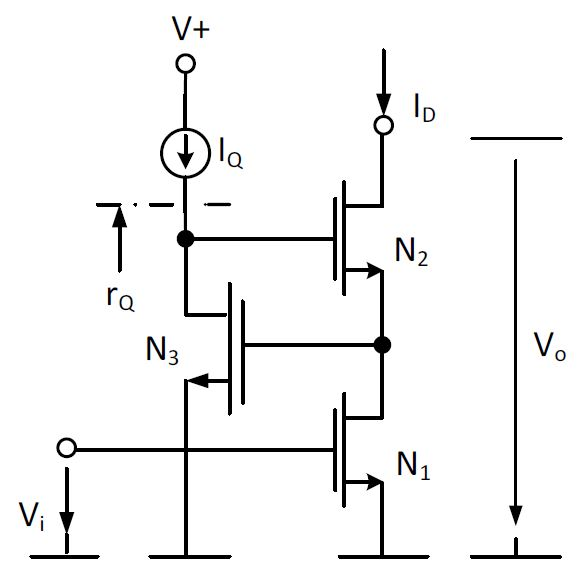
\includegraphics[height=4.5cm]{chapters/Stromquelle/images/geregelteKaskode}\\ \hline
\end{tabular} \\
\begin{longtable}{|l|l|l|}
	\hline
	\textbf{Konfiguration}&\textbf{Ausgangswiderstand $r_0$}&\textbf{min. Ausgangsspannung $V_{0,min}$}\\ \hline
	\endhead
	Einfache Quelle &$r_{out}=r_{iD}=r_{DS}=\frac{1}{g_0}=$&$V_0 > V_{0,min}=V_{DS,sat}$\\
	mit 1 Transistor&$\frac{V_A+V_{DS}}{I_D}\approx \frac{V_A}{I_D}$&\\ \hline
	Stromquelle mit &$r_{iD}=r_{DS}(1+\frac{R_S}{r_S}+\frac{R_S}{r_{DS}})=$&$V_0 > V_{0,min} = R_S I_D + V_{DS,sat}$\\
	Source-Widerstand&$\frac{1}{g_0}\left( 1+g_mR_S\right) + R_S$&\\ \hline
	Stromquelle mit Kaskode&$r_{out}=r_{o2}\approx \frac{r^2_{DS}}{r_{S2}}=$&$V_{0,min}=V_{G2}-V_{GS2}+V_{DS2,sat}$\\
	&$\left( \frac{r_{DS}}{r_S} \right) r_{DS}=\mu\cdot r_{DS}=\frac{1}{g_{o1}}\cdot\frac{g_{m2}}{g_{o2}}$ &$V_{0,min}=V_{DS1,sat}+V_{DS2,sat}$\\
	&&(mit $V_{G2}=V_{DS1,sat}+G_{GS2}$)\\ \hline
	Stromquelle mit geregelter Kaskode&$r_{out}\approx r_{DS1}\cdot\frac{r_{DS2}}{r_{S2}}\cdot\frac{r_{DS3}}{r_{S3}}=\frac{1}{g_{o1}}\cdot\frac{g_{m2}}{g_{o2}}\cdot\frac{g_{m3}}{g_{o3}}$&$V_{0,min}=2V_{DS,sat}$ \\ \hline
\end{longtable}